\section{数据库设计}\label{sec:Database_Design}

\subsection{设计考虑}

设计 PetJoy项目的数据库需要充分考虑平台的多样化需求,以确保能有效支持不同模块的功能。首先,针对用户和宠物信息的复杂性,我们在需求分析阶段明确了系统所需的数据类型和关系,包括用户账号管理、宠物领养、新闻资讯、社区互动等模块。通过详细的需求分析,我们确定了系统所需的关键数据结构,为数据库的后续设计奠定了基础。在逻辑架构设计中,我们将需求转化为具体的数据库实体和关系模式。这一过程中,我们考虑了各模块之间的数据交互和依赖关系,确保每个子系统的数据存储和访问能够高效且一致。例如,宠物领养模块需要与用户数据进行关联,社区互动模块需要处理用户发布的内容和评论,这些都在数据库设计中得到了充分体现。通过模块化的数据库设计,我们不仅实现了功能的扩展性,还确保了数据的一致性和完整性,能够支持 PetJoy 平台的长期可持续发展。最终,我们通过触发器设计和数据定义语言(DDL)的实现,进一步强化了数据库在操作过程中的安全性和可靠性。例如,触发器在用户操作如账号创建、内容发布等事件时自动执行预定义的操作,以确保数据的一致性和完整性。这些设计考虑使 PetJoy 平台能够在应对各种用户需求的同时,保持高效稳定的运行。

具体内容可以参考本项目数据库设计文档。

\subsection{逻辑设计}

数据库的逻辑设计包括数据库关系模式图、表设计、数据库设计和数据定义语言设计以及触发器设计。

\subsubsection{数据库关系模式图}

数据库关系模式图(\cref{fig:RelationshipSchema})的设计反映了本项目的信息系统。

\begin{figure}[htbp]
	\centering
	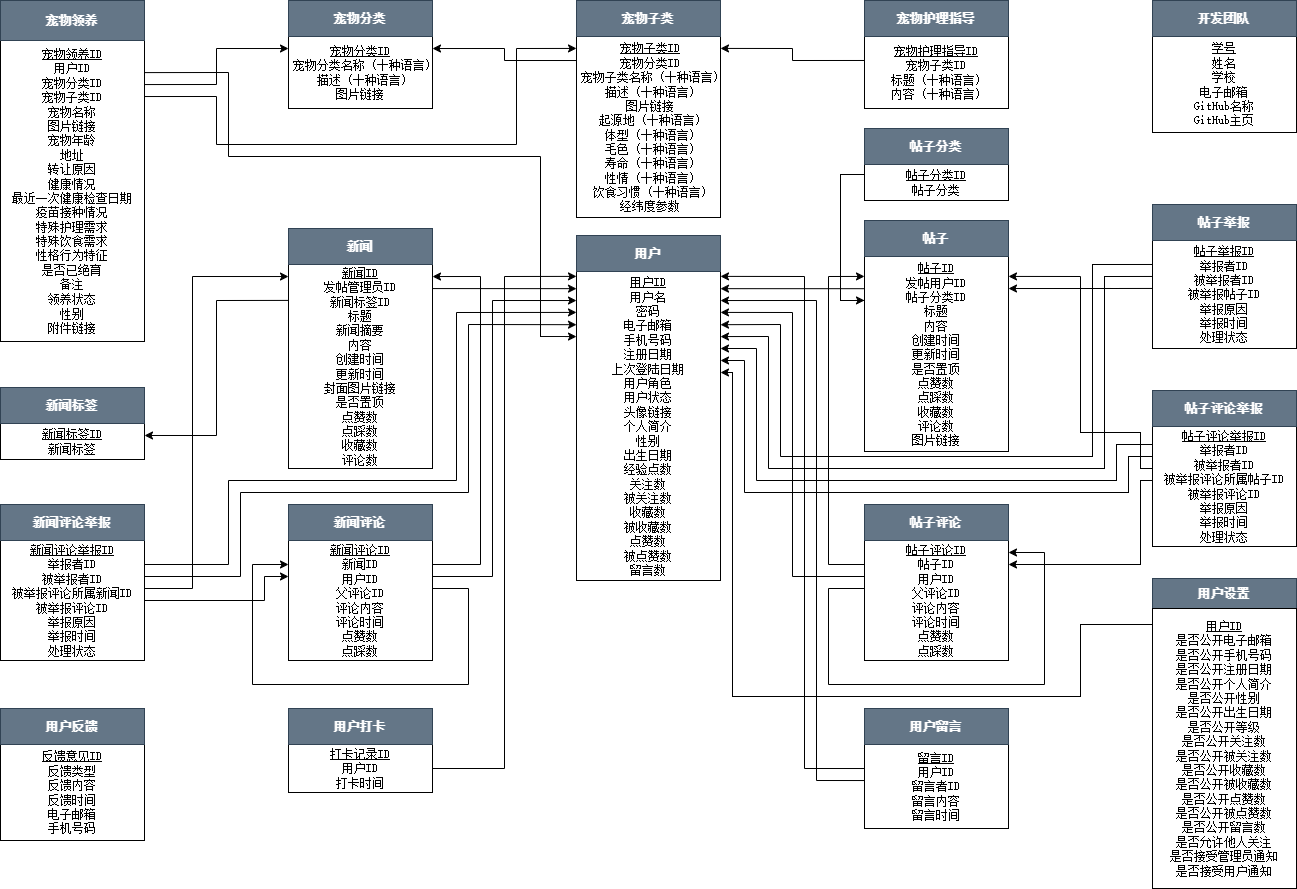
\includegraphics[width=\textwidth]{figures/RelationshipSchema.png}
	\caption{数据库关系模式图}
	\label{fig:RelationshipSchema}
\end{figure}

数据库的模块化设计通过将功能划分为独立的表,确保系统高度组织化和减少模块间依赖性,涵盖用户中心、内容管理、举报系统、通知系统、宠物领养模块和开发团队信息等关键模块。每个模块专注于特定功能,如用户信息集中管理、内容互动追踪、举报处理、信息通知、宠物领养分类管理,以及开发团队信息记录,整体设计优化了用户体验,增强了平台的互动性和信任度。

\subsubsection{数据库定义语言(DDL)设计}

在数据库设计过程中,确保数据定义语言(DDL)的有效实现是至关重要的。我们基于多方面的考量,对各个表进行了全面的DDL设计。这些方面包括但不限于:

\begin{itemize}
	\item \textbf{规范化}:通过对数据进行规范化处理,减少数据冗余,确保数据的一致性和完整性。
	\item \textbf{主键和索引}:为每个表定义合适的主键和索引,优化数据的检索速度和操作性能。
	\item \textbf{外键关系}:通过设置外键,确保表与表之间的关系得以正确表达和维护,实现数据的关联性。
	\item \textbf{数据类型与约束}:为每个字段选择最适合的数据类型,并通过设置约束条件(如非空、唯一性等)来确保数据的准确性和有效性。
	\item \textbf{安全性与隐私保护}:通过访问控制和加密技术,保护敏感数据,确保数据库的安全性与用户隐私。
	\item \textbf{性能优化}:在DDL设计时,考虑了性能优化策略,如分区、分表等,以提高数据库在高并发和大数据量情况下的响应速度。
	\item \textbf{数据持久化}:通过适当的存储策略,确保数据在数据库中的持久保存,防止数据丢失。
	\item \textbf{扩展性与可维护性}:考虑未来的扩展需求,设计了可扩展的数据库结构,并确保数据库设计易于维护和升级。
\end{itemize}

\subsubsection{触发器设计}

触发器设计包括针对用户的打卡、关注、留言、帖子、评论、点赞、收藏、新闻评论等多个表的插入和删除操作。这些触发器的作用是通过记录插入和删除操作,自动增减相关的经验点数、关注数、留言数、点赞数、评论数、收藏数等,以动态维护系统中的各类数据统计。每个操作都对应特定的增减数值,用于实时更新系统的相关数据。

\subsection{E-R图设计}

数据库总体E-R图见\cref{fig:GeneralERDiagram}。

\begin{figure}[htbp]
	\centering
	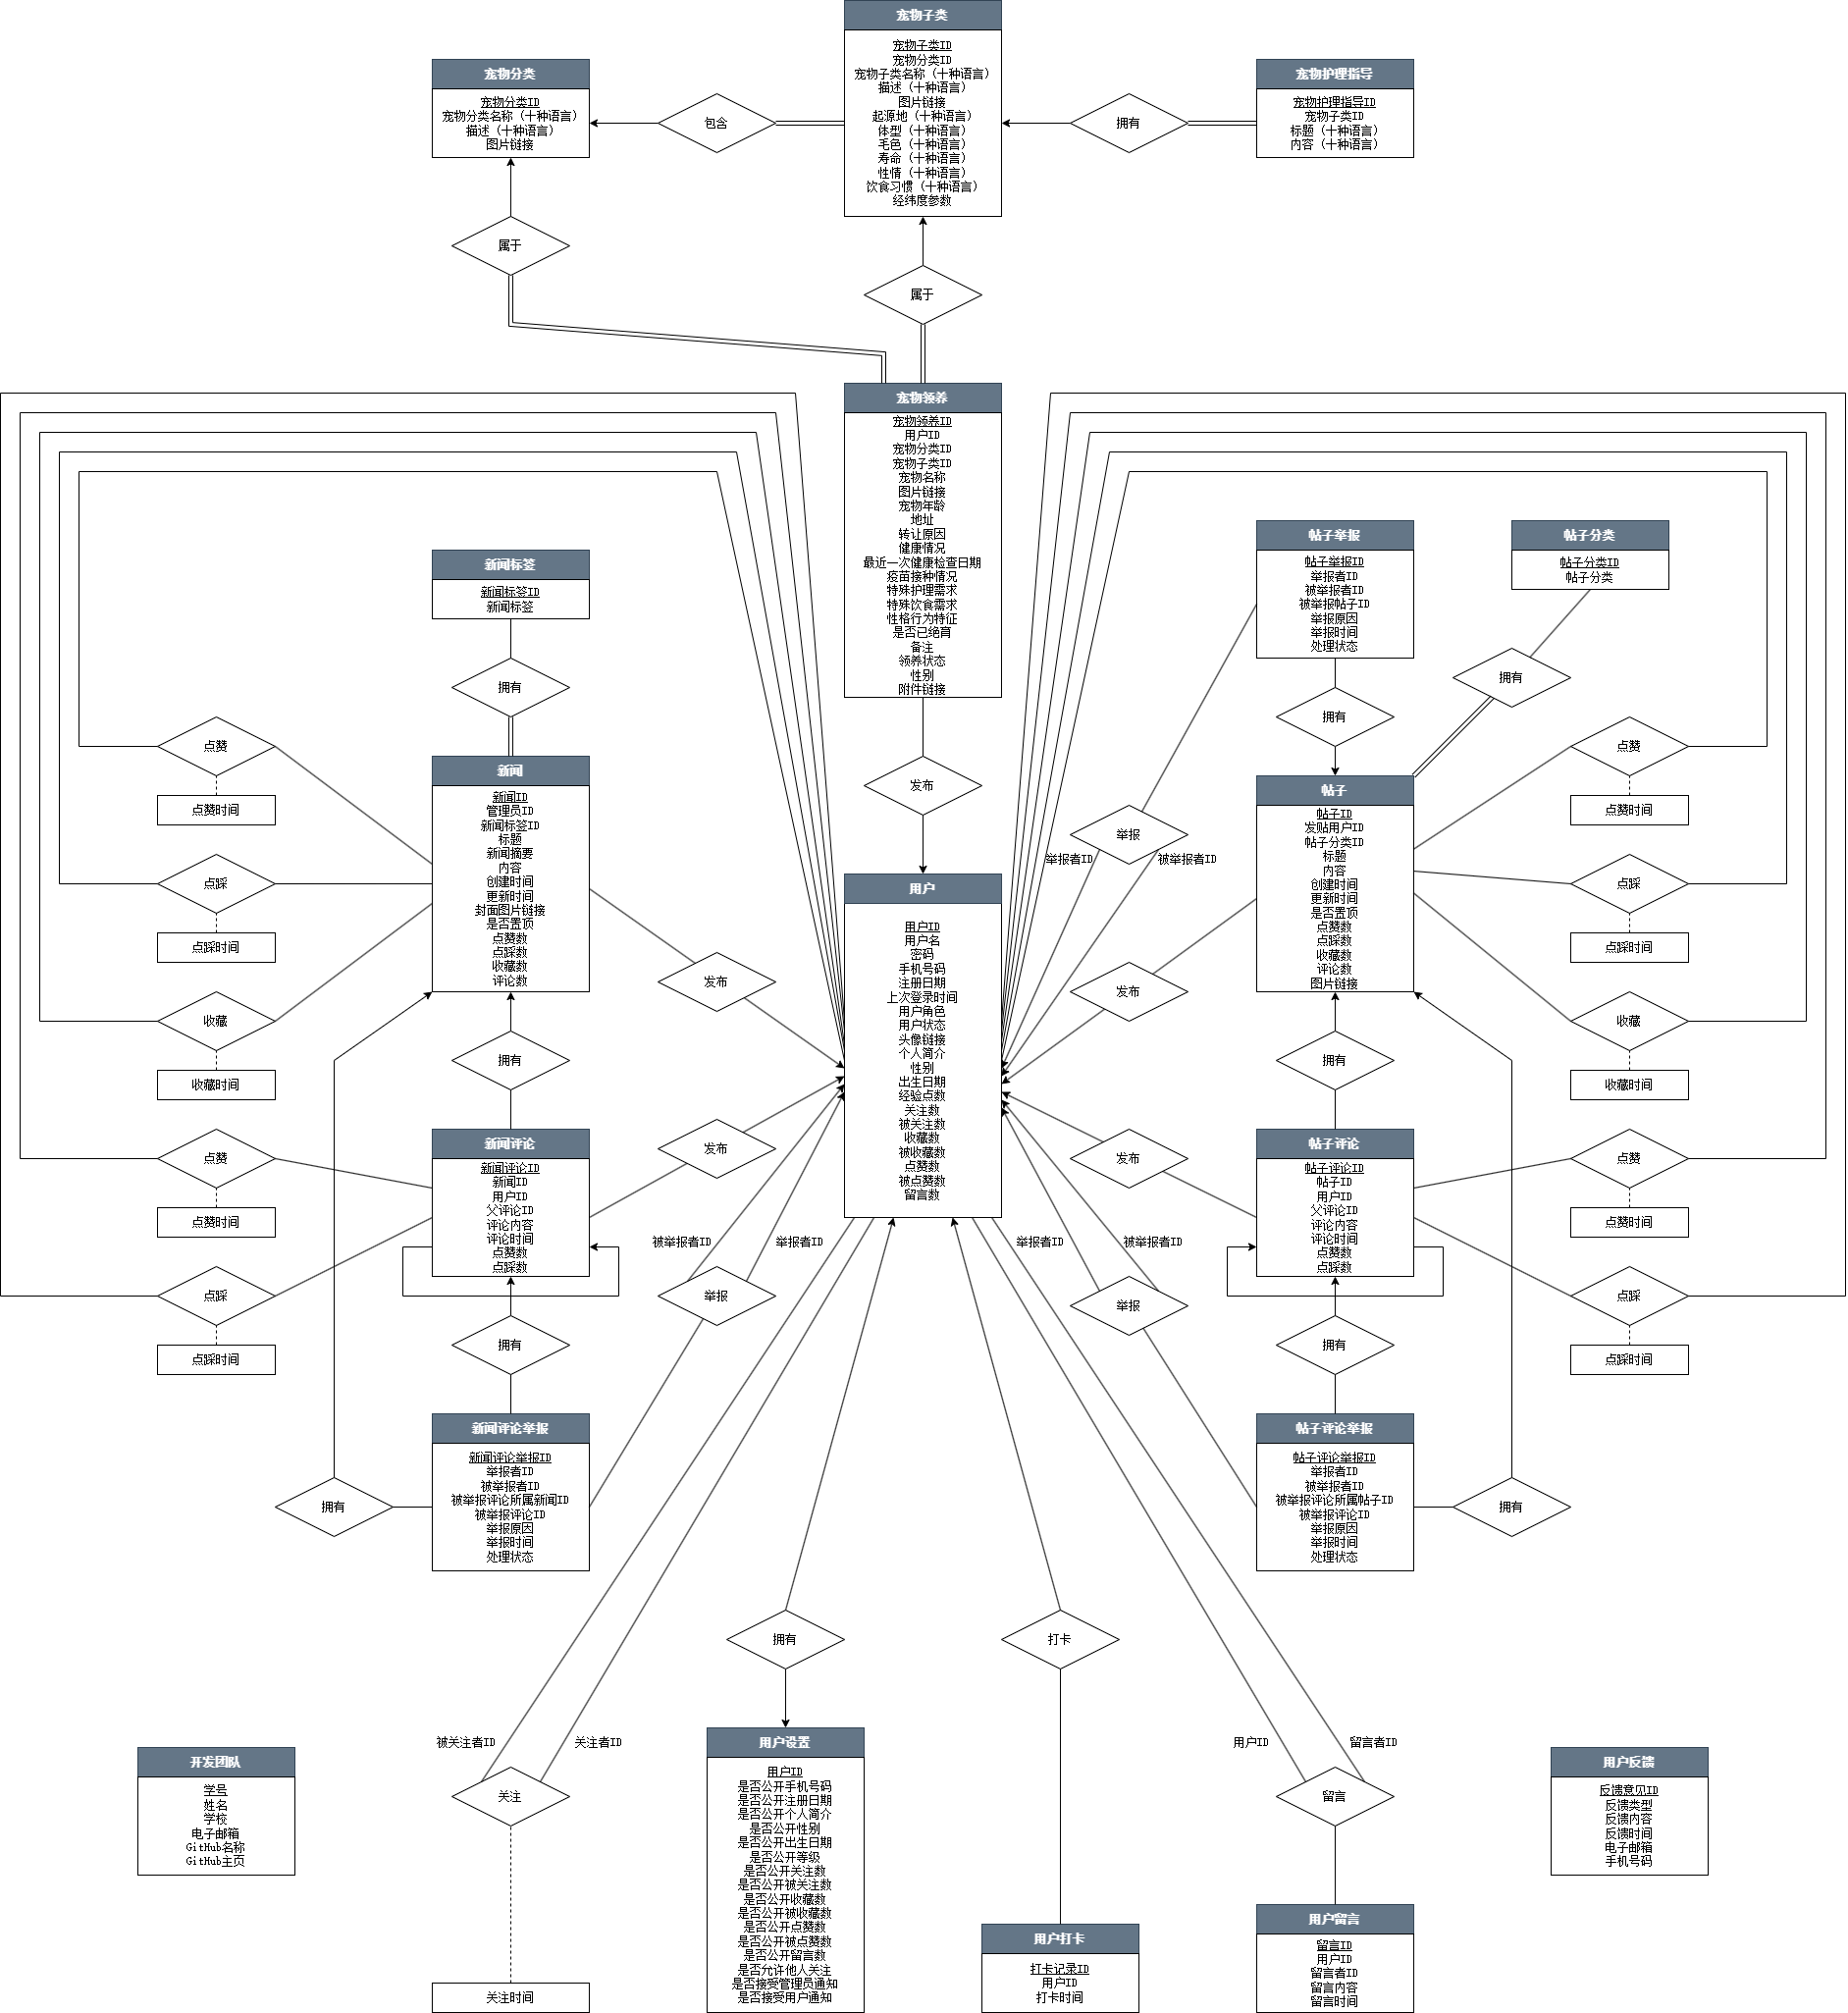
\includegraphics[width=\textwidth]{figures/GeneralERDiagram.png}
	\caption{数据库总体E-R图}
	\label{fig:GeneralERDiagram}
\end{figure}

数据库的总体E-R图作为宏观设计视图,全面展示了所有主要实体及其相互关系。该图涵盖了用户、帖子、新闻、宠物分类、宠物子类、通知等核心实体,并明确了它们之间的关系,如一对多和多对多的关联。例如,用户与帖子之间的多对一关系(一个用户可以发布多个帖子),以及帖子与评论之间的一对多关系(一个帖子可以有多个评论)。此外,总体E-R图还详细描绘了用户设置、用户关注、用户留言、新闻评论等更细致的功能关系。这种设计为理解数据库的结构和各个部分之间的交互提供了清晰的视角,也为数据库的实际建设和未来的数据操作提供了明确的指导。
\subsection{物理设计(表设计)}

我们一共设计了三十个表。其中包括用户表(USER)、用户设置表(USER SETTING)、用户打卡表(USER CHECK IN)、用户关注表(USER FOLLOW)、用户留言表(USER MESSAGE)、用户反馈表(USER FEEDBACK)、帖子分类表(POST CATEGORY)、帖子表(POST)、帖子评论表(POST COMMENT)、帖子点赞表(POST LIKE)、帖子点踩表(POST DISLIKE)、帖子评论点赞表(POST COMMENT LIKE)、帖子评论点踩表(POST COMMENT DISLIKE)、帖子收藏表(POST FAVORITE)、帖子举报表(POST REPORT)、帖子评论举报表(POST COMMENT REPORT)、新闻标签表(NEWS TAG)、新闻表(NEWS)、新闻评论表(NEWS COMMENT)、新闻点赞表(NEWS LIKE)、新闻点踩表(NEWS DISLIKE)、新闻评论点赞表(NEWS COMMENT LIKE)、新闻评论点踩表(NEWS COMMENT DISLIKE)、新闻收藏表(NEWS FAVORITE)、通知表(NOTIFICATION)、宠物分类表(PET CATEGORY)、宠物子类表(PET SUBCATEGORY)、宠物养护表(PET CARE GUIDE)、宠物领养表(PET ADOPTION)、开发团队表(DEVELOPMENT TEAM)。

设计三十个表的意义在于实现数据库的高度模块化和系统化管理,确保各个功能模块的独立性和灵活性,同时提升数据管理的效率和准确性。

\begin{itemize}
	\item \textbf{模块化设计}:每个表格对应特定的功能模块,例如用户管理、内容管理、举报处理、通知管理、宠物信息管理等。通过将功能细化为独立的表,可以有效降低模块之间的依赖性,便于系统的维护和升级。
	
	\item \textbf{数据组织与管理}:通过将不同类型的数据分离到专门的表中,系统可以更好地组织和管理数据,避免数据冗余,提高数据查询和处理的效率。这种设计也使得数据结构更加清晰,易于理解和操作。
	
	\item \textbf{扩展性与可维护性}:随着系统的成长和用户需求的变化,新的功能可以通过增加新的表或修改现有表的结构来实现,而不影响其他模块的正常运行。这种设计为未来的扩展和维护提供了良好的基础。
	
	\item \textbf{数据一致性与完整性}:通过合理的表结构设计和表间关系(如外键关联),系统能够确保数据的一致性和完整性,减少数据冲突和不一致的风险。这对用户体验和数据的可靠性至关重要。
	
	\item \textbf{功能的专注性}:每个表专注于处理特定类型的数据和操作,例如用户表管理用户的基本信息,帖子表管理用户发布的内容,举报表管理用户提交的举报信息等。这种专注性有助于提升系统的性能,并简化数据操作逻辑。
\end{itemize}






